\chapter{Introduction}

%suggest some unity to two disparate projects.  
Quantum mechanics is fundamentally a statistical theory, in that it only makes predictions for 
the probabilities of events~\cite{Sakurai1994}.
The probability for an event to occur is given by the Born rule, which says the probability is given by 
the absolute-square of the probability amplitude for that event.  
If there are multiple pathways by which an event can take place, the total amplitude for an event is 
the sum over the amplitudes for each possible pathways~\cite{Feynman1965}.  
These paths encompass paths through abstract spaces, such as the number of excitations in a field.
In this case, the intermediate particles correspond to are referred to as ``virtual particles'', 
which are referred to as quantum fluctuations.
This sum over intermediate amplitudes can lead to novel quantum effects such as the Casimir effect,
where electrically neutral, material bodies are attracted to each other due to the exchange of virtual photons.
%\comment{Perhaps Peres?}

Alternatively, the probabilistic nature of quantum mechanics implies that the results of quantum measurements 
are stochastic quantities which fluctuate under repeated measurements.  
This is particularly relevant as modern experiments can isolate single quantum systems for long 
periods of time and continuously measure their properties.  One can then think of reconstructing
the system's trajectory through time as it evolves based on the measurement~\cite{Carmichael1993}.  

This thesis presents two projects reflecting each aspect of quantum fluctuations.  
The projects are further connected by their quantum mechanical underpinning, the computational methods 
employed to simulate stochastic processes, and their relevance to modern experiments on atoms.  
The first project is a method of computing energies related to Casimir effect, while the second project is related to 
continuous quantum position measurements of atoms.  The majority of this thesis will be devoted
to the first project, with the second project being discussed in the final chapter.  
The key results presented in this thesis have been published in~\cite{
Mackrory2010, Mackrory2016,Mackrory2017a, Mackrory2017b}
% Through advances in modern experimental technology both of these categories of effect are now 
% directly observable.%~\cite{WisemanMilburn2010, Dalvit2011}.  

% The first project relates to computing Casimir forces via the worldline method, and occupies the majority
% of this thesis.  In brief, the worldline method is a Monte Carlo method for computing Casimir energies
% via ensembles of closed Brownian paths.  The work presented here extends the method by
%  developing analytical and numerical techniques to 

% The second theme will be using quantum trajectories to simulate continuous positions measurements on atoms.
% Both of these projects are related to fundamental quantum optical phenomena, 
% that we will explore using stochastic calculus, and Monte-Carlo methods for numerical simulations.  

The remainder of the introduction will expand on the physical origin, modern experiments, and theoretical
techniques for computing both Casimir effects, and then continuous quantum measurements.  

% \comment{There are two roles for the randomness here.
%   From one point of view, the randomness is an intrinsic part of quantum mechanics,
%  and thus naturally shows up in fluctuation phenomena like the Casimir effect, or in quantum measurements.
%   Alternatively, if we are considering these calculations for energy or evolution as large integrals,
%  then we can efficiently compute these integrals by randomly sampling from their dominant regions.
%   In this sense, the randomness shows up as a calculational tool.}

% \begin{enumerate}
% \item General thesis about quantum physics of atoms using computation.  
% \item Thesis covers numerical monte-carlo techniques, where random numbers used in simulation.
% \item First new method for computing electromagnetic Casimir energies.
% \item Second, continuous position measurements of atoms taking into account experimental constraints.  
% \item United in perspective of numerical work relying on Monte-Carlo techniques,
%  to explore quantum phenomena relevant to modern experiments and pushes toward future technology  
% \end{enumerate}

\section{Casimir Forces}% in general and physical interpretation}

The Casimir force is a primarily attractive force that arises between material bodies interacting via 
quantized fields.
The most important example of the Casimir effect is due to fluctuations in the electromagnetic (EM) field, 
where one can think of the electrons in a body emitting and absorbing virtual photons that can interact
with other bodies.  The interacting bodies can be pairs of atoms, 
macroscopic bodies such as metallic planes, or atoms and macrosopic bodies.
Alternatively, the Casimir effect can be attributed to the attraction between instantaneous dipoles forming.  
This interpretation is intimately related to the van der Waals force, where 
molecules with fluctuating dipole moments are attracted to one another.

\todo{Seems to choppy - should expand on classic Casimir computation as an example.}

Beyond their importance as manifestations of quantum field theory, Casimir effects are also 
important to a range of modern experiments and developing technologies.  Some of these experiments 
will be discussed further in Sec.~\ref{sec:expt_review}.  In order to describe these experiments,
a number of theoretical and computational approaches have been developed.  The most important of
these modern methods are the so-called ``scattering method'' and ``worldline methods''.
To date, the scattering method is the only general purpose numerical method available for computing
Casimir forces in arbitrary arrangements of bodies, while this thesis aims to expand upon the worldline method.  
In Sec.~\ref{sec:numerical_review} we will briefly discuss these methods.  

At the outset, we note that there have been a number of books published on the subject of Casimir forces 
in recent years.  This reflects the importance of Casimir forces to both physicists and chemists, as 
well as the advent of new experiments which have spurred the development of new theoretical methods.  
% Milonni's clear text on QED sets the Casimir force in context as one manifestation of the quantized theory of light~\cite{Milonni1994}.
% while Milton's text emphasizes using Green function methods for computing a number of consequences for 
% the Casimir effect for various fields, dimensions~\cite{Milton2001}.
There have been more recent where the state-of-the-art in both theory and experiments is discussed by practitioners --- 
notably in the volumes by Bordag~\etal\cite{Bordag2009}, 
and the collection editted by Dalvit~\etal\cite{Dalvit2011}.  
%\todo{Cite Vogel and Welsch~\cite{VogelWelsch2006}.  Also cite Buhmann~\cite{Buhmann2012-vol1,Buhmann2012-vol2}}
While this thesis emphasizes simple physical applications, the application of Casimir or 
van der Waals forces is also important to problems in surface physics and chemistry, as discussed in the texts by 
 Parsegian~\cite{Parsegian2006} and Israelachivili~\etal~\cite{Israelachvili2011}.

% The references in the following sections are given to emphasize the important results and calculations
% and set the basic context for Casimir effects.   In addition we will often use these results 
% as checks in our later work.  % Broader bibliographic surveys of the (vast) Casimir literature
% % are available from Milton~\cite{Milton-bib} and Babb~\cite{Babb-bib}.

\subsection{Atomic Forces}

In his 1873 Ph.~D thesis van der Waals found deviations from ideal gas behaviour~\cite{vanderWaals}.
These deviations can be understood as the atoms possessing a finite size, and experiencing forces between the gas atoms 
--- this whole class of forces inter-molecular forces are now referred to as van der Waals forces.
(A fuller account of the scientific history of these forces is discussed in Parsegian~\cite{Parsegian2006}.
While a number of different inter-molecular forces due to permanant
 or fluctuating electric dipoles are possible~\cite{Israelachvili2011},
we are primarily interested in forces due to fluctuating dipoles.  
This forces are typically referred to as London forces in honor of London's work
 using quantum mechanics to compute the potential between atoms via perturbation theory~\cite{London1930}.  
The potential has a characteristic $d^{-6}$ scaling.  As a heuristic argument, one can think of
 the first fluctuating dipole generating an electric field which decays as $d^{-3}$.  This field induces another
dipole in the other molecule.  The combined effect at the original atom scales as $(d^{-3})^2$.  

In 1948 Casimir and Polder extended this theory to using Quantum Electrodynamics
(QED) to account for the retardation due to the finite speed of light~\cite{CasimirPolder1948}. 
They found that in the far-field 
(where the transition wavelengths $\omega_A$ exceed the separation of the atoms $d$, $d\gg c/\omega_A$)
the interatomic potential decays more rapidly as $d^{-7}$.  The change in power law can be 
attributed to the induced dipoles decorrelating over the time-of-flight of the virtual photon, 
and thus having a weaker interaction.  
\todo{Is this from Milonni?}
Furthermore, they found an attractive force between an atom and perfectly conducting wall, with a $d^{-3}$ scaling
in the near field (van der Waals) regime, passes over to $d^{-4}$ scaling in the far-field.
In this case the atom can be thought of as interacting with it's image in the perfect conductor,   
which leads to an attractive potential for the atom,
\begin{equation}
  V_{CP}(d) =-\frac{3\hbar c\alpha_0}{64\pi^2\epsilon_0 d^4},
\end{equation}
where $\hbar$ is the reduced Planck's constant, $c$ is the speed of light, $\alpha_0$ is the atom's static polarizability,
and $\epsilon_0$ is the permittivity of free space.  Throughout this thesis we will refer to these
atom-wall type forces as Casimir-Polder forces.  

\comment{started transferred material}
This interpretation follows from taking the EM field Hamiltonian to be 
\begin{equation}
  E = \sum_k \hbar\omega_k\left(\op{a}^\dag_k \op{a}_k + \frac{1}{2}\right)
\end{equation}
where $\op{a}_k$ is the annihilation operator for mode $k$.  In the absence of any excitations only the 
constant term contributes.  
The Casimir-Polder energy can also be thought of in terms of emitting and re-absorbing photons.
In that case the interaction Hamiltonian is
\begin{equation}
  H_{\text{int}} = -\vect{d\cdot E} = -\sum_k(\sigma+\sigma^\dag)[a_kf^*_k(\hat{x})+a^\dag_kf_k(\hat{x})]
\end{equation}
\todo{Need free Hamiltonian for atom too.}
\todo{Also need mode functions}
These terms are normally dropped in the rotating-wave-approximation, as they 
are typically much smaller than the energy-conserving terms.  
\comment{dropped in material}

We can now present a schematic computation of the Casimir-Polder potential, with an emphasis 
on the broad techniques, intuition, and connections to other computations~(
 The discussion here follows Steck~\S{9.3} of Ref.\cite{SteckNotes}).  \todo{right period?}
This theory treats the interaction of the atoms with the light field via the interaction Hamiltonian
\begin{equation}
  H_{\text{int}} = -\frac{e}{mc}\hat{\vect{p}}\cdot\hat{\vect{A}}(\hat{\vect{x}}) + \frac{e^2}{2mc^2}
  |\hat{\vect{A}}(\hat{\vect{x}})|^2
\end{equation}
where $\hat{\vect{p}}$ is the quantum momentum operator for the atom, and $\hat{\vect{A}}$ is the 
quantized operator for the EM vector potential at the atom's position $\vect{r}$.  \todo{Expand field operators
$\op{A}(\vect{x},t) = \sum_k a_k e^{-i\omega_k t} f_k(\vect{x}) + \text{h.c}$}
(This interaction can instead be treated with $H_{\text{int}} = -\op{\vect{d}}\cdot \op{\vect{E}}$ where
these Hamiltonians are connected by the Power-Zienau transformation~\cite{SteckNotes}.\todo{Find page})
To find a non-zero effect one must go to second-order in perturbation theory, which leads to an atomic
energy shift to state $n$ of 
\begin{equation}
  V\subCP = \sum_{m\ne n,\vect{k}} \frac{
    |\langle E_n, 0|  H_{int}|E_m, 1_{\vect{k}}\rangle\langle E_m, 1_{\vect{k}}|  H_{int}|E_n, 0\rangle}{E_n-E_m-\hbar\omega_k},
\end{equation}
where $E_m$ are the atom's energy levels, the photon has energy $\hbar\omega_k$, 
and $\langle E_n,1_\vect{k}\rangle$ denotes the state with the atom in energy level $n$ and one photon in mode $\vect{k}$.
The shift $V\subCP$ can be understood as two transitions - from the ground state with no photons to an excited state with one photon,
and then transitioning back.  This is further summed over all possible intermediate states.
This process is represented schematically via the Feynman diagram in Fig.~\ref{fig:feynman_CP}, where 
an atom in the ground-state emits a virtual photon, and re-absorbs it.  This transition
is a ``virtual'' one, in that these intermediate states are not directly physically observable, 
but rather reflect the apparatus of quantum mechanical perturbation theory.
Note also that the photon is emitted into a mode $k$, 
where the allowed modes must satisfy the electromagnetic boundary conditions
on the surfaces of the bodies.  The resulting electromagnetic mode functions (and thus the potential)
are then sensitive to the arrangements of the bodies.  This is distinct from the case in most 
field theory calculations where the modes are described by plane waves.  
\begin{figure}
  \centering
\begin{fmffile}{atom-loop}
  \begin{fmfgraph*}(60,40)
    \fmfleft{i}
    \fmfright{o}
    \fmftop{t}
    \fmf{plain}{i,v1}
    \fmf{plain}{v2,o}
    \fmf{plain,label=$|e_j\rangle$}{v1,v2}
    \fmf{photon,left=0.5,tension=.4}{v1,vt,v2}
    \fmf{phantom,tension=1}{t,vt}
    \fmflabel{$|g\rangle$}{i}
    \fmflabel{$|g\rangle$}{o}
    \fmflabel{$|1_{\vect{k}}\rangle$}{vt}
  \end{fmfgraph*}
\end{fmffile}
\caption[Feynman Diagram for Casimir-Polder Energy]
{Feynman diagram representing an atom interacting with electromagnetic field via emitting and absorbing photons.  
  The wavy line represents the electromagnetic Green function in the presence of boundaries --- as opposed to the usual plane 
  waves exploiting in field theory computations.  The atom is excited into intermediate states.
}
\label{fig:feynman_CP}
\end{figure}

The Casimir-Polder energy shift can be split into a product of atomic and field pieces.  
It is often convenient for calculations to write the energy in terms of the imaginary frequency, $\omega = -is$,
since on the imaginary frequency axis, most functions of interest are smoothly decaying real functions.
\todo{Cite Johnson for benefits?  Kramers-Kr\"onig relations.}
To linear order in the coupling, the energy can be written on the imaginary frequency $is$ as 
\begin{equation}
  V\subCP(\vect{x}) = -\frac{\hbar c}{2}\int_0^\infty ds \alpha_{jk}(is)G^{(S)}_{kj}(\vect{r},\vect{r},is),
\end{equation}
where $\alpha_{ij}$ is the polarizability tensor, $G^{(S)}$ is the scattering part of the EM Green
tensor~\cite{McLachlan1963, McLachlan1963a}.
The scattering part of the Green function essentially subtracts off the vacuum 
EM Green function $G^{(S)}=G-G^{(0)}$ --- this is essentially renormalizing the energy
by subtracting off contributions that are independent of the bodies.  
This has the same from as a linear-response calculation~\cite{Altland2011}, finding the linear-response of the 
atom to it's interaction with the EM field.
In this case $\alpha_{ij}$ is the susceptibility of the atom responding to perturbations in the EM field.  
At this order of perturbation theory, the EM Green tensor is given by its classical counterpart,
which satisfies
\begin{equation}
  \nabla\times\nabla\times G(\vect{x},\vect{x'}) 
  + \frac{\omega^2}{c^2}\epsilon G(\vect{x},\vect{x'}) 
  = \omega^2\delta_{ij}\delta(\vect{x-x'}).
\end{equation}
 Evaluate at imaginary frequency. Note fully quantum theory, can account for atomic transitions.
\begin{equation}
  \alpha_{ij} = \sum_n\sum_m \frac{\langle E_n | d_i|E_m\rangle \langle E_m| d_j|E_n\rangle}{E_m-E_n}.
\end{equation}

While we have only given the linear energy shift, there are a number of higher loop contributions
which can be resummed analytically due to the relative simplicity of the expansion~\cite{Rosa2011}.  
\todo{Cite Dzyaloshinksii or papers book for resummation?}
The result of which is 
\begin{equation}
  V\subCP(\vect{r}) = \frac{\hbar c}{2\pi}\int_0^\infty ds \tr \log[I - \alpha(is) G^{(S)}(\vect{r},\vect{r})].
\end{equation}
This method of computing Casimir--Polder energies via classical Green functions has been expanded upon
in Ch. 7 of Milonni~\cite{Milonni1994}, Vogel and Welsch~\cite{VogelWelsch2006} and Buhmann~\cite{Buhmann2012-vol1,Buhmann2012-vol2}.

% \begin{enumerate}
% %\item Cite Lifshitz, Dzyaloshinski, Abrisokov.
% \item Cite Schwinger~\cite{Schwinger1978, Milton1978}  Scalar green functions.  
% \item Green tensor methods
% \item Cite Barton
% \end{enumerate}

\subsection{Forces between bodies: Casimir Energy}

The classic example due to Casimir~\cite{Casimir1948} predicts that a pair of electrically neutral,
perfectly conducting plates will attract one another due to their interaction with the quantized 
electromagnetic (EM) field.  
The presence of the conductors forces the electric field to vanish on the surfaces,
which restricts the allowed modes of the electromagnetic field, as illustrated in Fig.~\ref{fig:Casimir_sketch}.
Each quantized mode of the electromagnetic field contributes
to the energy, even in the ground state with zero photons.  Each mode contributes 
$E_\alpha=\hbar\omega_\alpha/2$ , where $\hbar$ is Planck's  constant, and $\omega_\alpha$ is the frequency of the mode.
The total energy is found by summing the mode for each energy --- the total energy is
badly divergent since each term in the sum is positive.  However a finite answer can 
be found by consider an energy \emph{difference} between two different configurations.  
The subtraction to eliminate divergences is a simple form of field theoretic renormalization, 
and will be essential in computations of Casimir quantities.  
In this case, the energy when the bodies are removed to spatial infinity is subtracted.  
The renormalized energy between the plates is
\begin{equation}
  E-E_0 = -\frac{\hbar c}{240\pi^2 d^3},
\end{equation}
where $c$ is the speed of light in vacuum, $\hbar$ is the reduced Planck constant,
and $d$ is the distance between the plates.  Note that in this expression there is no
mention of the material properties of the media --- this is an artifact of imposing Dirichlet
boundary conditions on the surfaces.  

\begin{figure}
\center
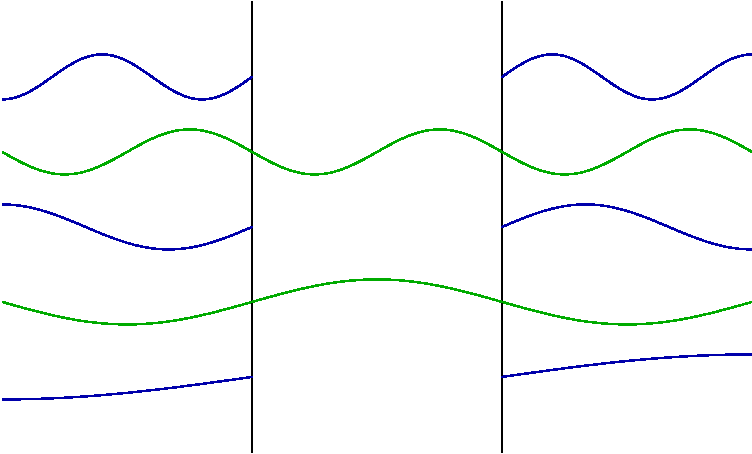
\includegraphics[width=6cm]{fig/intro/twoplanes_wave}
\caption[Allowed modes between parallel plates]
{Sketch of allowed modes between perfectly conducting plates. 
 Only waves with a half-integer number of wavelengths fit between the plates.
Blue modes are only allowed outside the plates, while green modes are allowed inside
and outside.  Modes have been vertically offset for clarity.  }
\label{fig:Casimir_sketch}
\end{figure}

The theory was extended by Lifshitz to describe forces between dielectric half-spaces~\cite{Lifshitz1956,
Dzyaloshinskii1959,Dzyaloshinskii1961}.
The Casimir force between two dielectric half-spaces of permittivities $\epsilon_1,\epsilon_2$
separated by a gap of thickness filled with permittivity $\epsilon_3$ is given by 
\begin{align}
\frac{F}{L^2} =& -\frac{\hbar}{2\pi^2c^3}\int_0^\infty d\xi \xi^3 \epsilon_3^{3/2}
\int_1^\infty dp\,p^2\sum_{s=\text{TE, TM}}
 \frac{r^{(s)}_{13}r^{(s)}_{23}e^{-2\sqrt{\epsilon_3}p\xi d/c}}{1 - r^{(s)}_{13}r^{(s)}_{23}e^{-2\sqrt{\epsilon_3}p\xi d/c}}
%\bigg[  \frac{r\supTE_{13}r\supTE_{23}e^{-2\sqrt{\epsilon_3}p\xi d/c}}{1 - r\supTE_{13}r\supTE_{23}e^{-2\sqrt{\epsilon_3}p\xi d/c}}
% + \frac{r\supTM_{13}r\supTM_{23}e^{-2\sqrt{\epsilon_3}p\xi d/c}}{1 - r\supTM_{13}r\supTM_{23}e^{-2\sqrt{\epsilon_3}p\xi d/c}}\bigg],
\end{align}
where the electromagnetic reflection coefficients are given by 
\begin{align}
  r\supTE_{ij} & = \frac{s_i-s_j}{s_i+s_j},\quad
  r\supTM_{ij} & = \frac{\epsilon_j s_i - \epsilon_i s_j}{\epsilon_j s_i + \epsilon_i s_j},
\end{align}
and
\begin{equation}
  s_i = \sqrt{p^2 + \epsilon_i/\epsilon_3-1}
\end{equation}
following Zhou~\cite{Zhou1995}.  As intimidating as this expression is, it can be heuristically derived with
relative ease via the ``argument principle''~\cite{vanKampen1968}.  
In essence, since the Casimir energy is the sum of the vacuum energy over all modes, the energy can
be written as a complex contour integral of the energy against a function with poles at the allowed 
energies.  For two plates the allowed modes satisfy the Fabry-Perot condition,
\begin{equation}
  \Delta = 1 - r_1r_2 e^{2ik d}.
\end{equation}

\begin{itemize}
  \item $E = \sum_k\frac{\hbar \omega_k}{2}$
  \item Should insert sum over transverse momenta.  This sum runs over all modes, not just frequency.
  \item Only allowed modes contribute.  
    Between two plates, the allowed modes must satisfy the Fabry-Perot criterion: 
    $\Delta = 1- r_1r_2e^{2ik_3d} =0$.
  \item Use fact that in complex analysis integrating function in closed loop in complex plane gets
    $\oint dz f(z) = 2\pi i\sum_{\text{poles} z_i}\text{Res} f(z_i)$.
  \item So energy can be written as 
    \begin{equation}
      E = \sum_k \frac{\hbar \omega_k}{2} = \oint dz \frac{\hbar z}{2(2\pi i)} \frac{\Delta'(z)}{\Delta(z)},
    \end{equation}
    where the function $\Delta'/\Delta$ is designed to have unit residue at the zeroes of $\Delta(z)$.
  \item Now integrate by parts w.r.t. $z$
    \begin{equation}
      E = \oint dz \frac{\hbar}{2(2\pi i)} \log\Delta(z).
    \end{equation}
  \item Now differentiate w.r.t $d$ to get force, and done.  
\end{itemize}
(Similar versions of this are used to derive scattering method results as well \todo{Cite correct Lambrecht paper for 2x2 matrices
in scattering formalism})

% This was further expanded on by Dzyaloshinskii~\etal\cite{Dzyaloshinskii1959,Dzyaloshinskii1961} who
% showed the connection between Casimir force and the pair-wise van der Waals potentials.  
This work is reviewed by McLachlan~\cite{McLachlan1963, McLachlan1963a}.  

The Casimir-Polder results for interacting atoms are recovered from the Lifshitz formula by taking the limit of dilute bodies,
$\epsilon \approx 1+\alpha n$, where $n\ll 1$ is the density.
In addition, the perfect-conductor Casimir can be found by taking $r\rightarrow 1$, and evaluating the 
integrals.

The Lifshitz theory can be extended to account for dispersion and finite temperature.  
Some care is required in quantizing the electromagnetic field within dielectric media,
since due to the Kramers-Kr\"onig relations, the presence of dispersion implies dissipation.
The usual approach to open-systems in quantum mechanics is to couple the system to a reservoir, 
and then trace out, or integrate out, the reservoir.
It has been phenomenologically observed that one gets the correct answers by a direct substitution
$\epsilon(\vect{x})\rightarrow \epsilon(\omega,\vect{x})$.  This issue has in investigated in~
\cite{Barash1975,Rosa2010}, and justified by careful examination of the thermodynamic energy
and relation to the microscopic details of the medium.   

\subsection{Physical Interpretation}

% However, boundary conditions are idealizations that ignore the structure
The Casimir effect naturally fits into the broader context of quantum field theory.  
Casimir initially framed the effect as a result of the zero-point energy associated with each mode of
the field.  

The Casimir effect is best thought of as a long-ranged interaction between dielectric bodies 
mediated via the electromagnetic field~\cite{Jaffe2005, Rahi2009}.
As Fig.~\ref{fig:Feynman-electron-action} shows, the Casimir effect can be thought of as the 
interaction of electrons on different bodies with one another via the electromagnetic field.  
We are interested in energies small relative to the binding energies of the dielectrics, and very weak
fields.  We can then use an effective description in terms of the coarse-grained linear-response of the 
medium to electromagnetic fields described by susceptibility $\chi$.  The susceptibility $\chi$
is found from the microscopic theory via linear-response such as the Kubo formula.
This view makes the clearest connection to the underlying physics, rather than emphasizing idealized
boundary conditions.  

\todo{Details of Kubo?}
\comment{Effective interaction: expanding out perturbation theory leads to $\langle j_\mu j_\nu\rangle$
correlation functions.  Via Kubo formalism for linear response, this is related to the conductivity
tensor $\sigma_{\mu\nu}$, which is in turn related to the dielectric constant $\chi$}

 \begin{figure}
 \centering
 \begin{fmffile}{wall-wall}
% \begin{fmfgraph}(50,30)
%  \fmftop{t0,t1,t2,t3}
%  \fmfbottom{b0,b1,b2,b3}
%  \fmf{fermion,tension=0.5}{t1,v1}
%  \fmf{fermion,tension=0.5}{t2,v3}
%  \fmf{fermion,tension=0.5}{b1,v2}
%  \fmf{fermion,tension=0.5}{b2,v4}
%  \fmffreeze
% \fmf{photon,tension=0}{v1,v3}
% \fmf{photon,tension=0}{v2,v4}
% \fmf{fermion,tension=0}{v1,v2}
% %\fmf{fermion,tension=0,left}{v2,v1}
% \fmf{fermion,tension=0}{v3,v4}
% %\fmf{fermion,tension=0,right}{v4,v3}
% \end{fmfgraph}
\begin{fmfgraph}(50,30)
 \fmftop{t0,t1,t2,t3}
 \fmfbottom{b0,b1,b2,b3}
 \fmf{phantom}{t1,v1}
 \fmf{phantom}{t2,v3}
 \fmf{phantom}{b1,v2}
 \fmf{phantom}{b2,v4}
 \fmffreeze
\fmf{photon}{v1,v3}
\fmf{photon}{v2,v4}
\fmf{fermion,tension=0}{v1,v2}
\fmf{fermion,tension=0,left}{v2,v1}
\fmf{fermion,tension=0}{v3,v4}
\fmf{fermion,tension=0,right}{v4,v3}
\end{fmfgraph}
\end{fmffile}
\caption[Casimir Energy in terms of fundamental QED processes. ]
 {Casimir Energy in terms of fundamental QED processes.  Electrons are considered bound within their respective media,
 but still interact with electrons on other bodies by exchanging photons.  The effective interaction of the 
electrons with the field is described by the dielectric constant.}
\end{figure}

% \begin{enumerate}
%   \item A number of interpretations.  Can attribute fluctuations to medium or fields.  
%     van der Waals fluctuating dipoles vs Casimir fluctuating EM fields.  
%     Atom/Bodies emitting and re-absorbing virtual photons.  
%   \item Zero-point energy.  
%   % \item Clearest physical picture is effective action from long-wavelength EM fluctuations 
%   %   interacting with matter.
%   % \item Emphasizes connection to underlying physics.  
% \end{enumerate}

\subsection{Distance and Energy Scales}

The Casimir force is typically most important between $1$nm and $10\mu$.  Below a
nanometer the continuum approximations used in computing the Casimir force begin to break down,
and a more careful condensed matter treatment would be required.  Above $10\mu m$, the force and 
energy become too small to measure. 

\subsubsection{Energy Scales}
We will compare the size of the Casimir force to typical Coulomb energies.  While 
the Casimir effect is short-ranged compared to the $d^{-1}$ Coulumb potential between charged particles.
However, most bodies are electrically neutral and thus have no long-ranged Coulomb potential, whereas
the Casimir effect applies even if the bodies have no net charge.

The typical Casimir--Polder energy scale can roughly be estimated from dimensional considerations.
For a typical atom, with size $r=1\AA$, the dipole moment $d\sim er$.  The static polarizability
is then $\alpha/sim \sum_jd_j^2/(\hbar\omega_j)$.
The Casimir-Polder energy in the far-field is then
\begin{align}
  V_{CP} &= -\frac{3\hbar c\alpha_0}{32\pi^2\epsilon_0 d^4}%\\
%  &= -\frac{3\hbar c e^2r^2}{32\pi^2\epsilon_0 \hbar\omega_0d^4}\\
%  &= -\frac{10^8 10^{-19}10^{-20}}{10^2  10^{-11} 10^{15}10^{-24}} eV\\
%  &= -\frac{10^{-31}}{10^{-19}} eV\\
  &\approx -10^{-12}eV,
\end{align}
which corresponds to a frequency shift on the order of $10$kHz for a generic atom at 1$\mu$m.  
In the near-field, it is necessary to shift over to the van der Waals energy.
As small as this energy is, in free-space it is the only attractive energy shift around for neutral atoms.

For macroscopic bodies we can compare the Casimir energy for perfect 
metal conductors at a distance $d$ to the energy stored in the capacitance.
The Casimir pressure (force per unit area) is $P_{\text{Cas}}=\frac{\hbar c\pi^2}{240 d^3}$.
This can be can be compared to the energy in a parallel-plate capacitor (pg. 219 of \cite{Milonni1994}.
For a parallel-plate capacitor, with surface charge density $\sigma$, the attractive force 
between the plates is $P_{\text{cap}}=\sigma^2/(2\epsilon_0)$.  For a parallel-plate capacitor filled with
vacuum, the capacitance is $C=A\epsilon_0/d = QV$, which implies $\sigma=Q/A=\epsilon_0V/d$.
The capacitive pressure is then $P_{\text{cap}}= \dfrac{\epsilon_0 V^2}{2d^2}$.  At a distance of $1\mu m$
this corresponds to a voltage of $17 mV$.  
Given that some experiments detect the Casimir force by balancing voltages, it is  quite important
to avoid even small voltages.  For conducting bodies there tend to be small fixed random distributions 
of localized electrical charge on the surface known as patch potentials.  For Casimir experiments, the patch potentials 
act as a long-ranged background that must be accounted for and subtracted away to extract
the more interesting Casimir energy.  

\subsubsection{Distance Scales}

The resulting attractive potential for bodies separated by a distance $d$ is a power law.
For pairs of macroscopic bodies the energy scales as $d^{-2}$--$d^{-3}$ for macroscopic bodies, 
while the energy scales as $d^{-6}$--$d^{-7}$ for pairs of atoms.  
The Casimir effect is important at distances around the resonant
wavelengths of the atom or medium, which are typically on the order of $1\mu$m for optical transitions.  
The Casimir effect is typically computed in a long-wavelength limit where the bodies can be treated 
as distinct from one another, or treat the material as being fixed.
This long-wavelength limit also corresponds to energies small compared to the binding energies of the bodies.
This approximation starts to break down for distances on the scale of the separation of the constituent atoms,
which is around $1$nm.  In addition, beyond distances of around $10 \mu$m, the Casimir effect is too
weak to detect.  

We can estimate typical distance scales by considering the dominant 
resonances of the medium, and the thermal wavelength.
 So the Casimir force is typically then important at distances below the
 transition wavelength which is usually around $1\mu m$.    
    
    Since the Casimir force is a broadband phenomenon, it depends on the resonant frequencies 
    of the interacting media, such as the atomic polarizablitiies $\alpha(\omega)$ or the dielectric
    function $\epsilon(\omega)$.  Furthermore at nonzero temperature, there is a thermal wavelength,
    $\omega_T=\kB T/\hbar$.  
    Given the radiative nature of the Casimir effect, there is a factor $e^{i\omega d/c}$ weighting the 
    frequency integrals.  This contributes most when its exponent factor is order one, and   
    the Lifshitz integral can be approximated in differing regimes.  

    In the near-field or van der Waals regime, the media are assumed to closer than the 
    resonant wavelength of the media $d\ll \omega_A/c,\omega_M/c$, the exponential factor 
    is unity, and each frequency contributes equally.  In essence, the interaction is an instantaneous 
    dipole interaction between the media.    

    The so-called Casimir-Polder regime occurs when the atoms are much further than a resonant wavelength 
    $d\gg \omega_A/c,\omega_M/c$,
    in which case the dominant contributions come at zero frequency, and the functions can be approximated
    with their static limit.  This far-field regime typically makes the potential decays more quickly.  

    Even further away from the bodies is the thermal regime $d\sim \omega_T/c$, where the real photons excited by the 
    thermal field contribute significantly.  In this regime the field decay is typically slower as $E\sim d^{-3}$,
    the same as the near-field van der Waals regime.  

\section{Summary of Casimir Experiments}
\label{sec:expt_review}
The Casimir effect has been measured in experiments, both for macroscopic bodies and atoms.
Beyond its interest as a fundamental quantum effect, the Casimir force is also important 
in designing novel physical devices for both atoms.

%Lamoreaux
\subsection{Casimir}
An early indirect measurement was liquid Helium flowing up the walls of a container.  
Lifshitz and co-workers applied the Casimir pressure to explain the phenomenon of liquid helium
flowing out of a jar.  The presence of the liquid helium crawling up the surface reduces the Casimir energy,
between the vacuum and the sides of the jar, so the liquid helium experiences an attractive pressure up the walls.  
\todo{Citation for this?}

While Casimir predicted an attractive force between neutral metal bodies in 1948,
it was only precisely measured in 1997 by Lamoreaux~\cite{Lamoreaux1997}.   
%Lamoreaux's work spurred a large amount of experimental and theoretical work.  
This experiment measured the Casimir force between a sphere above a metal plate,
and measured the force by detecting the change in capacitance of the arrangement.  
This landmark experiment was closely followed by measurement by Mohideen\etal\cite{Mohideen1998}
using an atomic force microscope to measure the force in a sphere-plate geometry.  
The Casimir force has also been directly measured in a nanoelectromechanical (NEMS) system 
by Chan~\etal~\cite{Chan2001}.  In this case, the Casimir force is detected by the modification it
makes to the frequency of a torsional oscillator suspended above a plate.  

The sphere-plate geometry has the experimental advantage of removing the need to carefully
align the metal plates. Given the strength of the Casimir force it is hard to keep the plates exactly parallel,
and separate, which is something that dogged early attempts to measure the Casimir force.
Despite the aforementioned difficulties, Bressi\etal measured the Casimir force between parallel plates~\cite{Bressi2002}.  
\comment{Lower precision?}

The Casimir force is also important in applications of microelectromechanical systems (MEMS), 
as a source of stiction~\cite{Tas1996, Serry1998, Buks2001}.  This is particularly important
in free standing structures such as nano-oscillators.  \todo{Comment on non-linear actuation blah?}
Given the Casimir force is an attractive potential, if parts of the device get too close to the substrate
they will permanently stick to one another, leading to device failure.  

Precisely measuring such a small force requires careful calibration of the measurements 
and removing systematic effects.  Two of the primary experimental errors are due to 
patch potentials, and surface roughness.  The patch potentials are localized surface 
charge distributions, which due to the longer range Coulomb interaction swamp the weaker
Casimir force.  Surface roughness reflects the fact the surfaces are not perfectly smooth,
and as such the exact distance between bodies is not clear.  While the roughness can be taken into
account in theory, the surface must also be carefully characterized.  Reviews of these and other 
difficulties are available~(for example, \cite{Dalvit2011}).

\subsection{Casimir-Polder}
%Skip over names?  
The Casimir-Polder force has been measured in the context of atomic beams, cavity QED, and 
Bose-Einstein condensates.  
In recent years technical advances and control over atomic systems have allowed the Casimir-Polder
force to be measured precisely.  

    The first attempts at directly measuring the Casimir-Polder force used atomic beams 
    near surfaces.  
    Sukenik~\etal made the first modern attempt to measure the Casimir-Polder force~\cite{Sukenik1993}.
    Their experiment passed a hot beam of atoms through an optical cavity and attempted to detect
    the effect by the small phase-shift induced on the atoms.  Unfortunately, their measurement 
    was not definitive.
    More recent experiments by Perreault~\etal\cite{Perreault2005}, and Lonig~\etal\cite{Lonij2009} succed in measuring
    the Casimir-Polder force with atomic beams.  These experiments passed an atomic beam past grating and 
    detected the phase-shift by atom interometry.  % These experiments act as precision tests of the theory,
    % and found that the first principles calculations based on perturbation theory are less successful
    % than an effective description informed by experimental data.  

    The Casimir-Polder effect has also been observed in the context of a Bose-Einstein Condensate (BEC)
    of ultra-cold atoms~\cite{Harber2005,Obrecht2007}.  The BEC allows for precise distance control,
    and can be used in atom interferometry to detect small phase shifts.    
    The atoms are confined to a harmonic trap, and can be brought near to a surface to probe the Casimir
    force.  The Casimir force acts to shift the oscillation frequency of the harmonic trap in a position
    dependent manner.  
    Furthermore, this technique was able to measure the Casimir force in the thermal regime, which
    is often difficult since the force is weak at those distance.  In this case it is easy to 
    vary the distance of the atoms from the surface from $1\mu m$ up to 10 $\mu m$ to observe
    the cross over between the Casimir-Polder and thermal regimes.

The Casimir-Polder force is also important in developing atomic technologies.  
There is a large effort across many fields to harness quantum technologies to develop scalable 
quantum devices for computation and simulation of quantum systems.  
Atoms are an attractive platform for a couple reasons.  
First, their internal states are well isolated from the environment which means they can have long coherence times.
Second, (for certain sub-species) their internal state can be precisely controlled via lasers.  
Atoms can also be cooled and trapped.  

    % \begin{enumerate}
    %   % \item Quantum computing offers to make certain computation tasks (most notably factorising 
    %   %   large prime numbers) and simulation taks much more efficient.  
    %   % \item Large push to develop scalable quantum devices in a number of model systems
    %   %   (NV centers, cold atomic gases).  Atoms provide excellent quantum memory, internal
    %   %   states are well isolated, controllable interactions via lasers.  
    %   \item 
    %   \item 
    % \end{enumerate}

    The Casimir-Polder effect is also important in the design of devices aiming to trap and interact
    with atoms near surfaces.  While ultra-cold atoms are very clean systems to work with for 
    studying and exploiting quantum effects, they are hard to minaturize and scale up.  In recent
    years there has been a concerted push to develop technology to regain the appealing features 
    of cold atoms in a scalable architecture. 

The desire to get strong-coupling between the atom and light fields, addressable qubits, and a scalable
architecture has pushed groups towards developing atomic traps that capture atoms close to dielectric surfaces.  
In this limit, the Casimir--Polder force is the dominant force, which can only be partially mitigated
by using laser fields to generate repulsive potentials.
  In designing these new devices it is essential to compute and account for the Casimir-Polder force
the atom's experience when brought close to the dielectric surface.  

    One direction that has been pursued is the so-called atom-chip~\cite{Folman2000,Schneider2003},
    where atoms are trapped near surfaces via a combination of lasers and magnetic fields from wires embedded in
    the surface.  The atoms are typically trapped within a micron of the surface.  
    In most applications the Casimir effect acts as a lower bound on how close bodies can be brought 
    to each other, which in turn limits the coupling strength and thus the speed of operation.  
    % In addition, the Casimir force as been taken into account in design 1D atom traps 
    % near a nanowire~\cite{Salem2010}.
    \todo{How close?  Limitations from CP?}

    Another direction that has been pursued is strong coupling of atoms to light via cavity 
    quantum electrodynamics (QED).  
    In order to address each atom, and ensure strong interactions, some groups 
    are developing microscopic dielectric waveguides to allow trapping, addressing and strongly interacting with a 
    single atom in a scalable manner~\cite{Alton2011, Hung2013, Goban2014}.  In this case
    the Casimir--Polder potential is explicitly accounted for as part of the trapping potential.
    \todo{More recent Kimble papers on this platform?}
    
% \item Antezza - chapters in Dalvit.  
% % \item Kimble atoms near toroidal resonators.
% %   Strongly Couple single atoms to optical field at single photon level.  
% %   Apply to toroidal resonators, and dielectric waveguides.  
% %   \cite{Alton2011}.
% %   Atoms above 1D Microcavity \cite{Hung2013}
% \item Atom-chips and atom-waveguids are attempts towards building scalable 
% architecture for quantum computer using atoms.
% Couple atoms to dielectric waveguides, and get stronger coupling (thus faster operation)
% by moving atoms more closely to couple to evanescent field.  
% \end{enumerate}
Challenges:  Need to characterize surface over broad frequency range.
Need methods with converge well for all geometries.  

\subsection{Current experimental directions}
\begin{enumerate}
\item Thermal casimir force
Sushkov\cite{Sushkov2011}.
Fight in literature over exact model used to describe metals at finite temperature.
Drude vs plasma model.  
 Lamoreaux favors Drude model, Capasso/Mohideen favours plasma model.
\item Repulsion (Cite Capasso experiment with bromobenzene).  Possibility of stable trapping
  if one could balance repulsion/attraction.  
 Metamaterials for repulsion.  (Can't work Rosa 2010/2011 since dielectric
  background dominates~\cite{Rosa2008}
  (Cite Vogel and Welsch chapter for Green function methods.  They cite 
  Feinberg and Sucher (1970) on pg 360 for repulsion)
  \item Search for repulsive forces as possible trapping (Motivation for this?)
  \item Can be found for magnetic media (but typically small).
    Metamaterials exhibit this for small range of frequencies.
    But Casimir broadband, and dielectric contribution ends up dominating.
    (\comment{ Cite Milonni on metametarials}.
    Sufficiently anistropic dielectric media (how anisotropic? \comment{Cite Milton})
    $\epsilon_1<\epsilon_3<\epsilon_2$ over a broad enough range of frequencies 
    \comment{Cite Lifshitz of liquid helium.
    Cite experiments, and note odd fluids.}.
    Geometries dependence (\comment{Cite reid paper on needle above hole}).
    
% Modifications to gravity on $1\mu m$ or $1mm$ scale.  Cite Lamoreaux 2000 Paper.  Gervaci?
% Yukawa type forces.  (Carrol's textbook on string theory dilaton.  
%  Subtract off Casimir force background.
%   Tino group.
%   Use Casimir shield with fairly thick gold to have same Casimir force, and thne vary the medium behind it.
%   Longer range gravity should lead to 
% Requires very careful measurements, on top of carefully extracting Casimir force.   


\end{enumerate}

The Casimir force is also important for speculative searches for new physics on the millimeter to micron
scale~\cite{Dimopoulos2003, Bezerra2011}.  The new physics must be shortranged, and is typically modelled as 
a Yukawa potential, $V_{\text{Yuk}}=\alpha e^{-\lambda r}/r$.  
On the micron scale however, the Casimir effect is the dominant interaction between neutral bodies,
 and must be carefully subtracted in an experimental procedure.
 However, one can look for deviations from the expected 
power laws, which has been used to exclude regions of the parameter space for the hypothetical
Yukawa interaction~\cite{Lamoreaux1997,Obrecht2007,Bezerra2011}.  
Experiments searching for modifications of gravity typically employ a thin gold layer over
a density modulation.  The gold layer provides a common short-ranged Casimir interaction, while the 
a density modulation allows measuring variations due to gravity~\cite{Sorrentino2009, Geraci2015}.
Given the difficulties in cleanly measuring the Casimir force, this even more ambitious program has yet 
to yield results.  

% \subsection{Chemistry/Helium/Geckos?}

% \begin{enumerate}
% \item Geckos use the Casimir force \cite{Autumn2002}.
% \item Military applications to mimic at human scale. Cite 2015 paper.   
% \end{enumerate}

\section{Path Integrals}

In order to discuss the modern methods of computing the Casimir effect it is necessary to introduce
the path-integral.

The path integral was originally developed by Richard Feynman as an alternative formulation of quantum mechanics
~(\cite{Feynman1948,Feynman1965}).  
In the path integral, the amplitude for a particle to propagate from one position to another,
is given by the sum over \emph{all} possible paths between the points.  
Each path is weighted with a phase $e^{iS[x(t)]/\hbar}$ where $S[x(t)]$ is the classical action for the path,
and $\hbar$ is the reduced Planck constant.   

    \begin{enumerate}
      \item Note connection - source of framing is Feynman, who used that reasoning to derive path
        integral
      \item Path integral is description of stochastic process.  Evolution of distribution described
        by wave-function.  Can think of randomly sampling from path integral, leading to stochastic 
        sample paths.  These correspond to Brownian motion for free quantum particle.  
      \item Brownian motion - non-differentiable, continuous paths.  Introduce Wiener paths.  
    \end{enumerate}
    
    Path integrals have been used extensively in a wide range of theoretical physics~\cite{Kleinert2012}.
    They form one basis for quantum field theory~\cite{Brown1994}, where they provide a 
    natural method for quantizing the relativistic gauge-field theories 
    that underly the Standard Model of particle physics~\cite{Srednicki2008}.
    In these field theoretic path-integrals, the integral runs over
    all possible field configurations connecting the initial and final states, and some care is required
    to handle the redundant degrees of freedom implied by gauge invariance~\cite{Fadeev1991}.

    Mark Kac worked with similar functional integrals, and put the path integral 
    on firmer mathematical footing~\cite{Kac1949}.  In Kac's work, and much of the mathematical
    work that followed, one weights each path
    by with $e^{-S_E[x]}$, where $S_E$ is the so-called Euclidean action.  
    This amounts to solving a diffusion equation, rather than the Schr\"odinger equation.  

    Path integrals have also been used in mathematics and statistics to describe stochastic 
    processes~\cite{Durrett1996, Karatzas1991}.  
    Can mathematically formulate a path integral as very high-dimensional integral.
    Can then use Monte-Carlo methods, to randomly sample from most important regions of integral.  

    They have even been used in studying quantum chaos---the study of the quantum analogues 
    of classically chaotic systems~\cite{Gutzwiller1990}.  In the semiclassical limit
    where the classical action $S[x(t)]$ is large, the path integral for a chaotic system
    can be approximated by only considering paths with periodic orbits.  \todo{Gutzwiller trace formula citation}

% \begin{enumerate}
% \item Found common use in field theory particularly for covariantly quantizing gauge field theories,
%  such as the Standard Model (cite Weinberg).  Integrate over all field configurations.  
% \item  Also related to stochastic processes, like Brownian motion \cite{Karatzas1991}.
% \end{enumerate}
  %   \comment{Should also cite Cecile Morette-deWitt, Kleinert and Grosche}.
    
  %   Wick-rotate Schr\"odinger equation to imaginary time, to get diffusion equation.
  %   Replaces oscillating Gaussian integrals for real, decaying ones.



\section{Computational methods for Casimir Effects}
\label{sec:numerical_review}

Although the Casimir force was explored by theorists before precision experiments were available,
the advent of precision experiments and new technologies has spurred developments in 
theoretical and computational methods.
While early work focused on highly symmetric geometries 
of bodies such as parallel planar bodies~\cite{Casimir1948} or spheres~\cite{Boyer1968}, 
current experiments require calculations for arbitrary shapes and arrangements of bodies, 
which have realistic material properties.  
This is a difficult task since the Casimir effect is a broadband phenomenon, depending on the whole 
range of frequencies.  Furthermore it depends sensitively on the geometry of the bodies involved, 
and one must carefully renormalize the results.  
For a simple, symmetric geometry it is possible to write down tractable analytical expressions for
the Casimir energy based on expanding the field in mode functions.  However for general geometries 
such an expansion may not be possible, or converge well.
These requirements force one to adopt a general numerical approach to computing Casimir forces~\cite{Johnson2011}.
We will discuss three of these methods: the proximity-force approximation (PFA), the scattering
or fluctuating surface current approach, and the worldline method.

% \begin{enumerate}
% %\item Experiments spurred development of theory.  
% % \item Prior methods relied on mode-function expansion of fields, which is only possible
% % for simple geometries.  
% % \item Theory must account for material properties.  Surface roughness.  
% % \item Need general methods, tend to result in numerical integrals.
% % \item Crudest method available is the proximity force approximation.  
% % \item Analytical theory based on green function methods.  (Russian school, McLachlan, Schwinger)
% % \item Scattering approach.  
% % \item Worldline method.  
% \end{enumerate}

\subsection{Proximity Force Approximation}

The proximity force approximation (PFA) is an uncontrolled approximation to
the Casimir force between generally shaped objects~\cite{Derjaguin1956}.  
\todo{Earlier citation is available}
The PFA treats each infinitesimal patch of the surfaces as if they were perfectly conducting planes,
and sums up the pair-wise interactions between different patches.
The PFA is assumed to be valid if the radius of curvature of the bodies $R$, is large relative to 
their separation $d$.  
For many years the PFA was the only practical general method of estimating Casimir forces.
The PFA has the advantage of being straightforward to implement, and functions as an order of magnitude
estimate for the Casimir force for arbitrary geometries.
It was used by Lamoreaux to estimate the Casimir force between the sphere-plate
in his landmark experiments, where the radius of the sphere was indeed large compared to the separations explored. 

However it has some prominent limitations.
First, it is only valid for vanishing curvature.
Second, the PFA assumes that the force can be found by integrating up
the pair-wise Casimir forces between each pair of surface patches.  This ignores the non-additivity
of the Casimir force.  Unlike the potential between electric charges where the total potential is
the sum of the pair-wise potential energies, the Casimir force for an arrangement
of bodies is not just the sum of the pair-wise energies.~(See \S{8.2} and \S{8.4} of \cite{Milonni1994}
Finally, the PFA allows only for strictly attractive forces.  
In contrast, the Casimir force can be repulsive, albeit under difficult to engineer circumstances 
such as media with a strong magnetic response, or anisotropic media.
\todo{PFA with frequency response for material?}

% \begin{enumerate}
% %\item Find first use?  Lamoreaux mentions usage.  Derjaguin?
% % \item Note problem with non-additivity. The PFA explicitly assumes that the force
% % can be found by adding up the pair-wise contributions from each surface patch.  
% % However, the Casimir force is a global phenomenon, and the total Casimir force
% % Useful if very limited curvature, or effectively approximate geometry as planar.  
% \item Only attractive.  (real electromagnetic casimir forces have possibility of 
% being repulsive, even if hard to realize in general.)
% \item ever extended to include material properties?
% \item Despite these limitations, the PFA is relatively straightforward to implement,
% and functions as an order of magnitude estimate for the Casimir force.  In the limit
% of vanishing curvature, the PFA converges to the correct Casimir force.  
% \end{enumerate}




\subsection{Scattering Approach}

The scattering approach is currently the only general method of computing 
electromagnetic Casimir forces betweenin general media.  The essence of the scattering method 
is encodes the presence of material bodies by the electric field they scatter.  

While originally developed as an analytical technique, 
the scattering method has also been converted to an efficiency numerical method.  

\begin{itemize}
  \item Note source of name - based on using scattering theory techniques for EM field.
\end{itemize}

It has been explored as an analytical technique,
and further converted to a form 
\begin{enumerate}
\item EM field depends on scattered field.  Encoded in reflection matrices
which are related to how EM field scatters from a given surface.  
\item Developed as analytical technique, and developed into general purpose numerical technique.
Numerous authors contributed over decades.
\end{enumerate}

\begin{enumerate}
  \item Developed as general method, for scattering between basis modes.  
    Initially used with analytical mode expansions.  Can also use finite element basis,
    much more adapted to arbitrary bodies.  
\item Physical picture is fluctuating currents on bodies.  Interact via EM field.
  Can use Green function as if dielectric suffused all space.  
Surface-Integral Equations (SIE) and Green's theorem relate surface integrals.  
\end{enumerate}

\begin{enumerate}

\item Cite Balian and Duplantier \cite{Balian1977, Balian1978}.
\item Cite Lambrecht and French collaborators
  \cite{Lambrecht2006, MaiaNeto2008,Canaguier-Durand2012}
%\item Cite Milton
\item Physical Picture based on generalized Green theorem from 
  SIE~\comment{Stratton}\cite{Stratton1941}.
\item Cite Bordag 1985 on quantization with delta functions?  There are others
Kardar and Li too.  \todo{Put in Borday1985, Kardar and Li citations}
\item Comment on Emig/Buscher showing you can use homogenous green function.
  Relation to Green's theorem.
\item Cite Emig,Jaffe,  and others for initial analytical techniques.  Relies on Green theorem.
\cite{Emig2004, Emig2007, Rahi2009}
\cite{Kenneth2006}
  Note use of existent analytical methods and similarities to existent 
  numerical FTDT techniques on earlier papers.  
  \cite{Rodriguez2007,Rodriguez2007a, Rodriguez2009}
% \item Cite Johnson/Reid for numerical progress.\cite{Reid2009,Reid2011, Reid2013}.
% \item Note success, applicability.  \comment{Cite experimental tylenol pill paper}
\end{enumerate}

The fluctuating-surface-current formulation is a general method for computing Casimir
energies for piece-wise continuous linear dielectric and magnetic media~\cite{Reid2009,Reid2011, Reid2013}.  
In essence the method calculates the interaction between electric and magnetic surface currents 
on different bodies, mediated by the EM field.  Mathematically this is derived 
from a path integral for the EM field, where the EM boundary conditions are enforced at the 
surfaces via functional $\delta$-functions.  The $\delta$-functions introduce fields 
bound to the surfaces, which can be interpreted as surface currents flowing to enforce boundary conditions.
After integrating out the EM field, these surface currents interact with one another via the EM
Green function.  Since the method assumes piece-wise, homogenous media and enforces EM boundary
conditions, it is the relatively simple homogenous EM Green function that appears in these expressions.
In order to discretize the method for numerical computations, a basis set to express the currents must
be chosen.  For general numerical methods, a triangular mesh is the most flexible.
The surface currents can also be formally integrated out, leaving the energy proportional 
to a functional determinant 
\begin{equation}
  E = \int_0^\infty d\xi \log\det\left[\mathbf{M}^{-1}_{\infty}\mathbf{M}\right],
\end{equation}
where $\xi$ is the imaginary frequency, 
and $\mathbf{M}$ is a matrix where the entires encode the scattering between various surface current 
elements via the homogenous EM green function,  
\begin{equation}
  M_{ab} = \int_{S_A} dx \int_{S_B} dy f_a(x) G_{ab}(x,y)f_b(y).
\end{equation}
\comment{Given general form, noting E/M coupling.  Also multiple bodies.  Renormalization kills
self-energy terms}
The $\mathbf{M}^{-1}_\infty$ term is a renormalization that subtracts the energy as the bodies are 
arbitrarily far apart, which acts to remove the energy from any self-interactions of the bodies with themselves.

Numerically, this method comes down to computing the determinant of a large sparse matrix, which is 
an intensive operation.  If a matrix has $N$ non-zero entries, the determinant requires $\order(N^3)$ operations
\comment{N rows or N entries?}.
While it is possible to parallelize computing the determinant~\cite{Beliakov2013}, 
this is difficult.
However, since each frequency $\xi$ contributes independently, the integral over $\xi$ could be
trivially parallelized.

The fluctuating-surface-current method has been used to 
for example describing the energy dependence of nanoparticles\todo{Find nanoparticle-scattering method citations}.
\todo{Note use in Kimble group for computing C-P potential}

\todo{Shortcomings?}

% \subsection{Modern Directions}

% \begin{enumerate}
%   \item Non-additivity of forces:  Reference for this?  What is the typical scale of the correction for non-additivity?

%   \item Search for repulsive forces

%   \item Casimir force important for stiction.
%   \item Attracts atoms, sets lower bound for how close you can get particles together.
% \item Dynamical Casimir effect/Unruh Effect?
%     \item Accelerating plate creates photons.  
%   \end{enumerate}

\comment{Vassilevich1998 has consistency conditions for boundary conditions
and gauge fixings}

\section{Scalar Worldline Casimir Energies}

The worldline method is an alternative method for computing Casimir energies.
The worldline method is a descendent of the scalar electrodynamics 
Feynman explored~\cite{Feynman1950}, where the effect of a quantum
field is described by summing over the paths of a particle interacting with the other bodies. 
\comment{Check!}
The worldline method was later developed as an alternative method for 
carrying out general quantum field theory calculations in terms of quantum particle 
mechanics~\cite{McKeon1993, Strassler1992,Schubert2001}.  
The worldline method is heavily based on Feynman's path-integral method, where the amplitude
for a particle to move from one position to another is the sum over all paths between the positions,
where each path acquires a phase proportional to the classical action for that path~\cite{Feynman1948,Feynman1965}.
The basic insight of the worldline method is that for one-loop effective actions, 
the field path integral calculation can be recast in terms of the particle path
 integral for particles travelling in closed space-time loops or paths.
  Higher order loop calculations can also be carried out with more particles, 
and gauge fields can also be treated~\cite{Schubert2001}.
  For example, the worldline method has been used to compute relativistic
 field effects for quantum electrodynamics (QED) such as the Lamb shift~\cite{Schmidt1995},
 and as a numerical algorithm~\cite{Mazur2014}.

Our primary interest in the worldline method is for computing Casimir energies, 
which was first used to compute scalar Casimir energies by Gies~\etal~\cite{Gies2003,Gies2006, Gies2006a}.
The scalar worldline method has been extended to finite temperatures~\cite{Klingmueller2008},
and used to study the torsion of inclined planes~\cite{Weber2009},
and forces in the sphere-plane and cylinder-plane geometries~\cite{Weber2010, Weber2010a}.  
The worldline method has also been applied to the Casimir piston, where there are interesting geometric effects
based on the geometry of the piston~\cite{Schaden2009,Schaden2009a}.


We consider a scalar field coupled to a background potential $V(\vect{x},t)$.  This potential
embodies the location of the bodies we are considering.  % Starting from the classical action,
% we will derive the Hamiltonian for the fields, and then compute the quantum partition function.  
% The partition function can be written as a path-integral, which is readily evaluated as a functional
% determinant.  Ultimately we want the free energy, which can be further converted into a path integral
% for a fictitious single-particle.  This single-particle path integral forms the basis of the numerical
% world line method.   

We now introduce the basic scalar worldline method, to discuss its positive features and limitations. 
Consider a scalar field $\phi(\vect{r},t)$, interacting with a background potential $V(\vect{r},t)$.  
The action for the field $\phi$ is given by 
\begin{equation}
  S = \int_0^T dt \int d\vect{r} \cL = \int_0^T dt \int d^{D-1}\vect{r} 
  \left[ \frac{1}{2c^2}(\partial_t\phi)^2-\frac{1}{2}|\nabla\phi|^2-V(\vect{r},t)\phi^2\right],
\end{equation}
where $V(\vect{r},t)$ defines the surfaces of the interacting objects
\begin{equation}
  V(\vect{r}) := \lambda \sum_r \delta[\sigma_r(\vect{x}-\vect{R}_r)],
\end{equation}
where $\lambda$ is the coupling constant, $\sigma_r(\vect{x})=0$ marks the locations of the surfaces, 
and $\vect{R}_r$ marks the center location of each body.
In most work on scalar worldlines, the coupling constant $\lambda$ is taken to infinity, 
which corresponds to imposing Dirichlet boundary conditions on the surfaces. 
In certain geometries this recovers electromagnetic 
Casimir results for idealized perfect conductors.  

From the Lagrangian, one can find the Hamiltonian and quantize the theory.
 (While this is a somewhat length procedure, it is the clear formal procedure for quantization,
 and useful to follow in cases where there may be ambiguities).
The momentum conjugate to $\phi$ is given by
\begin{equation}
  \Pi := \frac{\delta \cL}{\delta(\partial_t\phi)} = \frac{1}{c^2}\partial_t\phi,
\end{equation}
where $\frac{\delta}{\delta f(t)}$ denotes the functional derivative with respect to $f(t)$.    
The Hamiltonian can then be easily found,
\begin{align}
  H &:= \int d^3x\,(\Pi\partial_t\phi -  L)\\ 
  &= \int d^3x\,\bigg[\frac{\Pi^2}{2} + \frac{1}{2}(\nabla\phi)^2 +V(\vect{x},t)\phi^2\bigg].  
\end{align}
We are now in a position to quantize the theory by promoting the classical fields to quantum operators, 
$\phi\rightarrow \op{\phi},\, \Pi\rightarrow\op{\Pi}$.
The fields can be promoted to operators with equal-time commutation relations
\begin{equation}
  [\op{\phi}(\vect{x},t),\op{\Pi}(\vect{x'},t)] = i\hbar \delta(\vect{x}-\vect{x'}).
\end{equation}
In exactly analogous fashion to quantum mechanics, the overlap between states is given by 
\begin{equation}
  \langle \phi|\Pi\rangle = \exp\bigg[\frac{i}{\hbar}\int d^3x \phi(\vect{x})\Pi(\vect{x})\bigg].
\end{equation}

We can compute physical quantities of interest such as Casimir energies and forces
by taking suitable derivatives of the partition function. 
The quantum partition function for the field is 
\begin{equation}
  Z = \tr[ e^{-\beta\op{H}}] = \int d\phi \langle \phi| e^{-\beta \op{H}}|\phi\rangle,
\end{equation}
where we have evaluated the trace over the complete set of field states.  
It is actually more useful to carry out calculations with the free energy $\mathcal{F}=-\kB T \log Z$.
In classic path-integral fashion the exponential operator can be split into $N$ pieces, and resolutions of the identity
in both fields and conjugate-momentum fields can be inserted between each piece.  

% \begin{align}
%   Z &= \int d\phi_0\prod_{n=1}^N d\phi_n \langle \phi_n| e^{-\Delta \beta \op{H}}|\Pi_n\rangle
%   \langle\Pi_n| \phi_{n-1}\rangle
% \end{align}

After integrating out the momentum fields, the partition function can be written as 
Euclidean Path integral (Generating Function) 
\begin{equation}
  Z = \int D\phi \exp\left\{-\int_0^{\hbar\beta c} d\tau \int d^3r
    \left[ \frac{1}{2}(\partial_\tau\phi)^2+\frac{1}{2}(\nabla\phi)^2+V(\vect{r})\phi^2\right]\right\},
\end{equation}
where $\tau=\beta\hbar c$.  The partition function can be cast into a more suggestive form
by integrating by parts in the exponential integrand, 
\begin{equation}
  Z = \int D\phi \exp\left\{-\int_0^{\hbar\beta c} d\tau \int d^3r\,\phi(\vect{r},\tau)
    \left[-\frac{1}{2}\partial_\tau^2-\frac{1}{2}\nabla^2+V(\vect{r})\right]\phi(\vect{r},\tau)\right\},
\end{equation}
where the surface terms can be discarded by assuming the fields tend to zero at spatial (and temporal)
infinity.\comment{Actually need frequencies for periodic functions.  Especially for finite temperature,
dispersion.  Will discuss more carefully later.}

The functional integral over $\phi$ is Gaussian and can be formally evaluated immediately as a 
functional determinant, since the differential operator is positive operator.  
Some care is required in regularizing such infinite determinants.
This is done in analogy with finite dimensional Gaussian integrals.  
We can consider treating the fields as only being evaluated on a finite lattice of space-time points, 
with the lattice also having a finite extent which bounds all bodies.  
The gradient operators 
can be treated via their finite difference approximations, which can be thought of as sparse matrices.
The limit of an arbitrarily large volume, and lattice resolution can be taken after integration.

In an analogous fashion, one can formally evaluate the partition function path integral as a 
functional determinant, 
\begin{equation}
  Z \propto {\det}^{-1/2}\left[-\frac{1}{2}\partial_\tau^2-\frac{1}{2}\nabla^2+V(\vect{x})\right].
\end{equation}
Note that the original computations for the worldline method stressed computing the quantum effective
action for the scalar field.  This yields essentially the same expression.  This expression has
also retained a factor of $2$ on the gradients --- this will simplify the representation of the 
worldline path integral.
The proportionality it due to an additional (infinite) normalization constant, which will
shortly be dealt with.  

The free energy for the interacting field can be written as 
\begin{equation}
  \mathcal{F} = -\kB T\log Z = \frac{1}{2}\kB T 
\log\det\bigg[-\frac{1}{2}\partial_\tau^2-\frac{1}{2}\nabla^2+V(\vect{x})\bigg].
  \label{eq:free-energy-det}
\end{equation}
As it stands this expression is divergent, however we will renormalize by subtracting off the 
same expression with the bodies removed to spatial infinity.  Physically this corresponds to 
computing energy differences between different configurations.  The renormalization also cancels off 
the inifite constant normalization factors.  

The free energy can now be converted into a single-particle path integral via some formal 
manipulations.  First we will use the identity $\log\det A=\tr\log A$, which can be readily
verified for positive finite matrices.  
\begin{align}
  \log\det A &= \log\prod_j \alpha_j
  =\sum_j \log\alpha_j
  = \tr\log A,\label{eq:log-det}
\end{align}
where we used the facts that the trace and determinant of a matrix are given by the sum
and product of its eigenvalues respectively. \comment{Check Kirsten/Vassilevich for better argument/citation}
Furthermore, we will use the integral representation of the logarithm,
\begin{equation}
  \log A -\log B= -\int_0^\infty \frac{d\cT}{\cT} (e^{-A\cT} - e^{-B\cT}),\label{eq:integral_log}
\end{equation}
where $A$ and $B$ are positive operators (i.e. $A$ and $B$ have strictly positive eigenvalues).
This expression also relies on a difference of terms to cancel out divergent terms at $T=0$.  The 
earlier renormalization by subtracting off the vacuum energy provides exactly this subtraction. 

By applying Eqs.~(\ref{eq:log-det}) and (\ref{eq:integral_log}) to free energy~(\ref{eq:free-energy-det}),
 the renormalized free energy can be rewritten as
\begin{equation}
  \mathcal{F}-\mathcal{F}_0 = -\frac{\kB T}{2}\int_0^\infty \frac{d\cT}{\cT}
  \tr\Big[e^{(\partial_\tau^2+\nabla^2)\cT}\big(e^{-\cT V(\vect{x})}-1\big)\Big].
\end{equation}
At this point, we introduce an $D$-dimensional auxiliary Hilbert space to evaluate the trace, where 
$\langle \vect{x},x_{\tau}| \op{p}_i|\psi\rangle = -i \partial_i\langle \vect{x},x_{\tau}|\psi\rangle$,
$[\op{x}_i,\op{p}_j]=i\delta_{ij}$.  

\begin{equation}
  \mathcal{F}-\mathcal{F}_0 = -\frac{\kB T}{2}\int_0^\infty \frac{d\cT}{\cT}
  \int d\vect{x}_0d\tau_0 \langle \vect{x}_0,\tau_0|e^{-(\op{p}_\tau^2+\op{\vect{p}}^2)\cT}\big(e^{-\cT V(\op{\vect{x}})}-1\big)
  |\vect{x}_0,\tau_0\rangle.
\end{equation}



The free energy is then in the form of the imaginary-time transition amplitude for a quantum particle
in $D$ space-time dimensions, in a potential $V$.  

\begin{itemize}
  \item Introduce auxiliary hilbert space.
  \item This is exactly the (imaginary-time) transition amplitude for a quantum particle.
  \item Same derivation as before.  Operators -> eigenvalues
  \item Carrying out Gaussian momentum integrals.
\end{itemize}
    
Worldline path integral
  \begin{equation}
    F = - \int \frac{dT}{T^{1+D/2}} \dlangle e^{-\cT\langle V\rangle} - 1\drangle,
  \end{equation}
  where $\cT$ is the loop proper time, $\langle V\rangle$ is the average of the potential 
around a particular loop, and $\dlangle\cdots\drangle$ denotes an ensemble average over Brownian paths.  

% We can compute the partition function for the field by Wick rotating to
%  imaginary time (or finite temperature), where the partition function is now given by 
% \begin{equation}
%   Z = \int D\phi \exp\left\{-\int_0^T dt \int d^3r 
%     \left[(\partial_t\phi)^2+(\nabla\phi)^2+V(\vect{r},t)\phi^2\right]\right\},
% \end{equation}
% The Gaussian integration over fields can be formally carried out as a functional determinant.
%   In order to compute the energy we need the logarithm of the partition function,
%  and various derivatives of it.
%   The end result of these manipulations is that the renormalized energy can be written as 
% \begin{equation}
% E_{\text{scalar}} = \frac{\hbar c}{(2\pi)^{D/2}}\int_0^\infty \frac{d\cT}{\cT^{1+D/2}}
%  \int d\vect{x} \dlangle e^{-\cT\langle V\rangle} -1\drangle,
% \end{equation}
% where $\cT$ is the loop ``time'' and governs the extent of the loops,
%  $\vect{x}_0$ is the loop starting point, $\dlangle \cdots\drangle$ denotes 
% an ensemble average over closed Gaussian random walks, 
% and $\langle\cdots\rangle$ denotes the average of a quantity around the loop.  

\begin{figure}
\center
\includegraphics[width=10cm]{fig/intro/hit_strong_coupling}
\caption[Schematic of worldline paths interacting with plane and sphere]
{Upper loop touches both objects and will contribute to Casimir energy.
  Lower loop only touches one body, and does not contribute to Casimir energy.}
\end{figure}

\begin{enumerate}
  \item Semi-classical approach to Casimir force via trace formula~\cite{Schaden1998}
  \item Also the optical path-integral \cite{Scardicchio2005, Scardicchio2006}.
\end{enumerate}

\subsection{Numerical method}

%\item Cite Schubert~\cite{Schubert2001}, Strassler~\cite{Strassler1992} on general worldline
% \begin{enumerate}
% %\item Summarize Strassler.  Can compute QFT effects from worldline path integrals.  
% % \item One loop effective actions can be described as single-particle worldline path integrals.  Can apply for higher order loops, and gauge fields, Cite Schubert.    
% % \item Cite QED at one loop order paper.  Get same results.  
% % \item Note similarity to Schwinger's trick for handling loop integrals in QED.  T is Schwinger's proper time.  
% \end{enumerate}
\begin{itemize}
  \item Generate ensemble of closed Brownian paths.
  \item Can be done by decoupling Gaussian integrals - so-called ``v-loop'' algorithm.
  \item Can also create open Brownian walk, then force to close by pro-rating final position around walk.
  \item Corresponds to IR vs BT?

  \item Due to renormalization, integrand is only non-zero if touch both bodies.
  \item In strong coupling limit (which is typically all that is explored) integrand goes to one if touch
    both bodies.  
  \item For given unit path, and position $x_0$ can find first touching time.  Then integrate over 
    positions and times.  For simple geometries this can be done analytically.  
\end{itemize}


  \subsection{Advantages and shortcomings of the scalar method}
\begin{enumerate}
  \item Advantages

  \begin{enumerate}
    \item Intuitively appealing picture of fluctuations moving through space-time.
      However - fictious time, no relativistic speed limits.  
    \item Algorithm is geometry independent, and no spatial or temporal grid.
      Instead have path resolution.  
      Generate paths, and see if they touch.
  \item Trivially parallelizable since each trajectory is independent. 
      Computation time scales as one /resources.  
  \end{enumerate}

  \item Shortcomings
    \begin{enumerate}
      \item No coupling of photons to medium.
      \item A scalar, not vector electromagnetism.
      \item Idealized boundary conditions.  
      \item No way to extract atomic energies.  (quick guess of suppressing spatial integral turns 
        out to be wrong direction).
    \end{enumerate}
  
\end{enumerate}

Thus far the worldline method has only been developed for scalar fields, 
without direct application to electromagnetic Casimir problems, 
other than for some speculation~\cite{Aehlig2011}.
  Currently, the potentials reflect the imposition of Dirichlet boundary 
conditions on the surfaces of the bodies, rather than a physical dielectric.
   In our work we will show how to incorporate the dielectric explicitly, 
and show how in simple geometries a new version of the scalar theory applies
 to electromagnetic problems.  

Others have made models in the static limit by ignoring the fluctuations in the field,
and focusing purely on the electrostatic energy.
 Similar functional determinants to worldline methods are found,
 and are evaluated explicitly using a spacial grid~\cite{Pasquali2008}.  

\subsection{Motivation and goal for thesis project}

Given those shortcomings, can we extend the scalar worldline method to vector electromagnetism.
Ideally we would retain the attractive features of the method, such as geometry independence of the paths,
simple path generation, and Monte Carlo sampling, while improving the method to account for the two physical polarization
states of the EM field, and properly account for the material properties of the medium.  

As this thesis will show, we have partially met those goals.  
% \begin{shaded}
%   The presence of $\delta(\vect{x}_N-\vect{x}_0)$ leads to an overall normalization constant $(2\pi\cT)^{-(D-1)/2}$.
%   This follows either from Hormander's argument, that 
%   \begin{equation}
%     \int d^nx\, \delta[h(\vect{x})]f(\vect{x}) = \int_{h^{-1}(0)} dS\,\frac{1}{|\nabla h(\vect{x})|}f(\vect{x}),
%   \end{equation}
% where $S$ is defined as the surface satisfying $h(\vect{x})=0$, and 
% $|\nabla h(\vect{x})|=\sqrt{\sum_k \left(\frac{\partial h}{\partial x_k}\right)^2}$.
%   In our case, we are restricting a sum of $N$ Gaussian integrals to have zero total.
%   If we define the increments $d\vect{x}_n = \vect{x}_{n+1}-\vect{x}_n$, then the loop constraint is $\delta(\sum_{k=0}^{N-1} \vect{x}_k)$.
%   If we account for the remaining normalizations of the $\vect{x}_n$ integral, then the normalization for the loop path integral is $\sqrt{2\pi\Delta \cT N} = \sqrt{2\pi\cT}$.  
% \footnote{See pages 826-828 of Dan's notes.}
% \end{shaded}


\section{Continuous Quantum Measurements}

Describe open quantum systems, and include information from continuous measurements. 

\begin{enumerate}
\item Quantum measurements are inherently probabilitistic.  
\item Thus, sequences of measurements are also inherently random.  
\item Greater experimental control means we can now probe isolated quantum systems repeatedly and see how they evolve.  
\item Move beyond simple projective measurements, which cannot describe things like position measurements,
    or absorbtive measurements like photon detection.  Once photon is measured it is destroyed.
\item To describe continuously weakly probing a system, also use stochastic processes as part of
    numerical simulation strategy.
\item Quantum tajectories correspond to monitoring a quantum system (like an atom) via a probe,
 for example shining light on the atom. \cite{Carmichael1993}
\item Simulated trajectories are possible trajectories a system could trace out as we observe.
  Also given a particular measurement record, they correspond to our best estimate of the current state of the system.  
\end{enumerate}

\begin{enumerate}
\item Cite Carmichael Rice JOSA paper~\cite{Carmichael1989}
\item Carmichael 1991 ~\cite{Carmichael1991}
\item Open Systems approach to Quantum Optics\cite{Carmichael1993}
\begin{enumerate}
  \item Motivated by photodetection, and modelling experiments developed a new approach to open systems.  
  \item Sample trajectories then correspond to actually results.
  \item Naturally fits Bayesian framework for interpretation of quantum state.  
\end{enumerate}

\item Example: Monitoring State of Two level atom.
\begin{enumerate}
  \item Hamiltonian and operators
  \item  Stochastic Schr\"odinger equation
    \begin{equation}
      d|\psi\rangle = -\frac{i}{\hbar}\op{H}|\psi\rangle dt 
      - \frac{\Gamma}{2}(\sigma^\dag\sigma-\langle \sigma^\dag\sigma\rangle)|\psi\rangle dt
      + \left(\frac{\sigma|\psi\rangle}{\langle \sigma^\dag\sigma\rangle^{1/2}}-|\psi\rangle \right)dN
      \end{equation}
    where $dN$ is Poisson process which is zero or one, with mean rate
    \begin{equation}
      \dlangle dN\drangle = \Gamma \langle \sigma^\dag\sigma\rangle dt.
    \end{equation}
    If Poisson process fires then detected emitted photon, which implies atom emitted photon, and should 
    apply lowering operator.  If no photon detected, then less likely to be in excited state.  
    Not only possible unravelling.  Can do homodyne detection - interfere light from atom
    with local oscillator.  Can extract phase info about atomic dipole.  Often necessary since direct
    detection typically has weak gain.  Interference effect amplifies the signal to detectable levels.
    However note EMCCD cameras can resolve/detect single photons - will form core of that part of thesis.
    Aspect of contextuality - type of measurement apparatus determines what can be inferred about the 
    state of the system.
 \item   Note that using $\dlangle\cdots\drangle$ for ensemble average over stochastic processes,
    and $\langle A\rangle:=\tr[A\rho]=\sum_i p_i \langle \psi_i|A|\rangle\psi_i\rangle$ 
    for quantum mechnical average.  
    \item Interpret photon detection or non-detection as gaining knowledge about state of system.
  \item Can get regular master equation by finding stochastic master equation, and tracing over noise.
  \item Crucial to use stochastic calculus to consistently work to $\order(dt)$.
  \item Path integral interpretation - master equation evolution is given by path integral, sum over all
    paths.  Monte-Carlo sampling of paths given quantum trajectories. 
    Note this was pointed out by Howard.  
\end{enumerate}
    
\item Cite Marte, Zoller, Parkins, Gardiner (MCWF)  \cite{Dalibard1992,Dum1992,Gardiner1992}
\item Cite Holland ~\cite{Holland1996}, Meystre~\cite{Greenwood1997}.
  Applied to position measurements of atoms by detecting photons.
  Detection of photons localizes atoms.  
\item Control Theory.~\cite{Wiseman1993} 
\begin{enumerate}
    \item Cite Wiseman book
   \item Jacobs and Doherty.
  \item Continuously monitoring system to implement closed-loop feedback control.  
  \item Feedback control to generate Fock states (Haroche group)
\end{enumerate}
\item Quantum Chaos
\begin{enumerate}
  \item Idea of exploring quantum-classical transition.
  Strong measurement is more classical.
  Can extract Lyupanov exponents for diverging trajectories.
  \cite{Bhattacharya2000,Habib2002,Habib2006}
  \cite{Scott2001}
  \item Theoretically shown.  As yet, this transition  not yet observed.  Need to develop
    theory in direction of more carefully modelling experiments.  
\end{enumerate}
\item Advantages:
\begin{enumerate}
  \item Computationally efficient as simulating wave functions.
  Take ensemble average at the end to get density matrix.  
  \item Natural form for feedback control and reconstructing trajectory.  
\end{enumerate}
\item Comment: Relationship of measurement with state and process tomography?  Any?  

\item Warshawski and Wiseman.
  Can describe additional uncertainty by including classical Bayesian probabilities for each indistinguishable trajectory.
  Note thesis of J. Thorne describing model for EMCCD camera.
  Given number for each pixel have probabilities for each number of photons.
  Must then incoherently average over all possible detection histories consistent with measured record.
  \cite{Warszawski2002,Warszawski2003a,Warszawski2003b}
\item Also cover results for generalized measurement functions and 
    somewhat surprising notion that particle reflects from a sufficiently
    strong quantum measurement.~\cite{Mackrory2010}
\end{enumerate}

\section{Thesis outline}

The rest of this thesis is laid out as follows:  In Ch.~\ref{ch:EM_quantization} we formally quantizing
the EM field in media, and derive the worldline expressions for the electromagnetic Casimir energy.
We will carry this out both for splitting the EM field into two non-interacting scalar polarizations,
as well as the fully coupled path integral.
We will also review others work on quantizing the EM field in media.
In Ch.~\ref{ch:feynman_kac} we will discuss the general methods of solving single-particle path 
integrals.  In particular, this relies on the Feynman-Kac formula, which states the path integral
 is the solution to a diffusion equation.  In simple cases, the Feynman-Kac formula can be solved,
and we will derive those solutions for some simple planar geometries. 
In Ch.~\ref{ch:analytical} we will use the results from the previous chapter to derive analytical 
results showing agreement between the worldline method and prior results, at least for planar media.
We will also discuss the transition between high and low temperature, and near-field within the
worldline context.  
In Ch.~\ref{ch:numerical} we discuss the numerical methods for evaluating worldline path integrals
This will includes efficient methods for computing gradients, as well as Monte Carlo sampling methods
for generating paths. 
In Ch.~\ref{ch:general} we will discuss the prospects for a general method based on the current
results and examine both an approximate method coupling the two polarizations together as well
as the fully coupled path integral method.  (We will test this for a mixed geometry for which
there are other tested methods to compare the worldline method against. 
In Ch.~\ref{ch:trajectory} we change topic to discussing continuous position measurements 
of single atoms.  We will derive the quantum trajectories for this case, and develop the framework
to account for variable measurement strength, and how to reconstruct the atomic trajectory
given the output of a realistic camera.  
Finally, we will summarize our findings in the conclusion.  


% \begin{enumerate}
% \item Background for path integrals, scalar worldlines, and EM field quantization.
% \item Cover 
% \item Analytical methods and computations in simple geometries.
% \item General method and numerical results.
% \item Shift to quantum trajectories.  
% \end{enumerate}



%%% Local Variables: 
%%% mode: latex
%%% TeX-master: "thesis_master"
%%% End: 